% Licensed under the Creative Commons Attribution Share Alike 4.0 International.
% See the LICENSE file in the repository root for full license text.

\begin{problemset}
	\item 探索 \lstinline{scanf}。输入以下程序。

	\begin{lstlisting}[language=c]
#include <stdio.h>

int main()
{
	int a, b;
	scanf("%d,%d", &a, &b);
	printf("%d, %d\n", a, b);
}
	\end{lstlisting}

	\begin{enumerate}
		\item 改编该程序,在末尾额外输出第 6 行的 \lstinline{scanf} 的返回值。
		\item 输入 \lstinline[showspaces=true]{114,514},程序输出了什么,\lstinline{scanf} 的返回值是多少?
		\item 同上一小问,但输入 \lstinline[showspaces=true]{114, 514}。(\lstinline[showspaces=true]{ } 表示空格)
		\item 同上一小问,但输入 \lstinline[showspaces=true]{114 514}。
		\item 调试程序,输入 \lstinline[showspaces=true]{114,},然后点击“全部中断”(图 \ref{pic:pause}),“调用堆栈”窗口中有什么内容?利用“自动窗口”记录变量 \lstinline{a} 和 \lstinline{b} 的值。

		\begin{figure}[H]
			\centering
			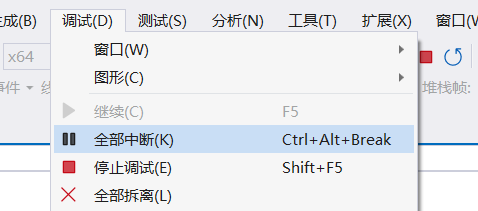
\includegraphics[width=0.5\linewidth]{pic/pause.png}
			\caption{调试时的“全部中断”功能}
			\label{pic:pause}
		\end{figure}
	\end{enumerate}

	\item 高级语言中,我们常写:
	\begin{lstlisting}[language=c, numbers=none]
a = a + 1
	\end{lstlisting}

	在 C 语言中,这样的表达式可以简写为:
	\begin{lstlisting}[language=c, numbers=none]
a += 1
	\end{lstlisting}

	称类似于 \lstinline{+=} 的运算符为\textbf{自反赋值运算符}。

	\begin{enumerate}
		\item 自反赋值运算符。自反赋值运算符在语法上与赋值运算符类似。将以下代码的第 4 行拆分成等效的 4 条\textbf{普通}赋值语句。

		\begin{lstlisting}[language=c]
int main()
{
	int a = 0, b = 0, c = 0, d = 0;
	a += b += c += d += 1;
}
		\end{lstlisting}

		提示:为了便于理解题意,下面给出答案的第一条语句。

		\begin{lstlisting}[language=c, numbers=none]
d = d + 1;
		\end{lstlisting}

		\item 按位异或。对于\textbf{只有一位}的二进制数,\textbf{异或(xor)}运算的真值表为:
		\begin{table}[H]
			\centering
			\begin{tabular}{c|c|c|}
				& 0 & 1
				\\\hline
				0 & 0 & 1
				\\\hline
				1 & 1 & 0
				\\\hline
			\end{tabular}
		\end{table}

		即相同为 0,不同为 1。按位异或的含义是,将两个二进制整数的每一位依次进行异或运算,在数学上用“$\oplus$”符号表示。例如:
		$$
		\begin{matrix}
			& 0001~0001
			\\
			{\oplus} & 0000~1011
			\\\hline
			& 0001~1010
		\end{matrix}
		$$

		C 语言中,按位异或用 \lstinline{^} 运算符表示。阅读下面的代码。

		\begin{lstlisting}[language=c]
int main()
{
	int a = 114, b = 514;
	a ^= b ^= a ^= b;
}
		\end{lstlisting}

		将以上代码的第 4 行拆分成等效的 3 条普通赋值语句,并调试拆分后的程序。程序运行到 \lstinline{main} 函数的右大括号时,变量 \lstinline{a, b} 的值分别是多少?\lstinline{a ^= b ^= a ^= b} 的功能是什么?
	\end{enumerate}

	\item 大括号对应的汇编指令。回答下面的问题。

	\begin{enumerate}
		\item 调试时,\lstinline{main} 函数的左大括号(\lstinline{{})可以单独地被当前行箭头指示(图 \ref{pic:brace}),原因是它对应了一些有用的汇编指令。\lstinline{main} 函数的左大括号对应的汇编指令的作用是什么?

		\begin{figure}[H]
			\centering
			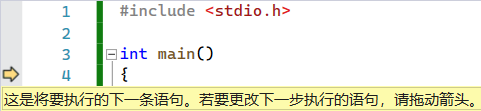
\includegraphics[width=0.75\linewidth]{pic/brace.png}
			\caption{\lstinline{main} 函数的左大括号成为当前行}
			\label{pic:brace}
		\end{figure}

		\item 调试时,\lstinline{main} 函数的右大括号可以单独地被当前行箭头指示。\lstinline{main} 函数的右大括号对应的汇编指令的作用是什么?

		\item 调试时,\lstinline[language=c]{if} 语句的左右大括号都不能单独地被当前行箭头指示,说明它们不对应任何汇编指令。而在 \lstinline[language=c]{if-else} 语句中,哪些大括号对应了汇编指令?这些汇编指令的作用分别是什么?从高级语言的角度描述这些作用。
	\end{enumerate}

	提示:此处所谓“对应”,是由你使用的编译器规定的,不是金科玉律,不要死死记住。本题的目的是熟悉 C 语言 \lstinline[language=c]{if-else} 语句的执行细节。

	提示:你可以调试下面的代码。

		\begin{lstlisting}[language=c]
#include <stdio.h>

int main()
{
	int a;
	scanf("%d", &a);
	if (a)
	{ // 它对应汇编指令吗?
		printf("if clause\n");
	} // 它对应汇编指令吗?
	else
	{ // 它对应汇编指令吗?
		printf("else clause\n");
	} // 它对应汇编指令吗?
}
		\end{lstlisting}

	\item 三目运算符。若某运算符只有一个操作数,则称之为单目运算符,例如负号运算符(\lstinline{-A})。同理,像减号(\lstinline{A - B})这样的运算符被称为双目运算符。C 语言支持的唯一三目运算符是 \lstinline{?:},其语法形如:
	\begin{lstlisting}[language=c, numbers=none]
A ? B : C
	\end{lstlisting}

	\lstinline{?:} 被称为\textbf{条件运算符},其含义是,先计算 \lstinline{A},如果 \lstinline{A} 为真(非零),则计算 \lstinline{B},并将 \lstinline{B} 的计算结果作为整个运算符的计算结果;如果 \lstinline{A} 为假(零),则计算 \lstinline{C},并将 \lstinline{C}  的计算结果作为整个运算符的计算结果。

	\begin{enumerate}
		\item 阅读下面的程序。

		\begin{lstlisting}[language=c]
#include <stdio.h>

int inc()
{
	static int count;
	return count = count + 1;
}

int main()
{
	int temp = inc() ? 0 : inc();
	printf("%d\n", inc());
}
		\end{lstlisting}

		该程序会输出什么?

		提示:运行程序后,在控制台中可以看到程序的输出。

		\item 如果不存在三目运算符,也能写出运行效果相同的程序,方法是使用 \lstinline[language=c]{if-else} 语句。不使用三目运算符,改写以下代码,使得程序的运行结果在任何输入下都保持不变。

		\begin{lstlisting}[language=c]
#include <stdio.h>

int main()
{
	int a;
	scanf("%d", &a);
	int to_output = a == 114514 ? 114 + 514 : 114 - 514;
	printf("%d\n", to_output);
}
		\end{lstlisting}

		将你的答案与以上代码进行对比,你认为三目运算符的作用是什么?

		\item 运算符具有优先级,我们熟知乘除法的优先级高于加减法的优先级。将以下 C 语言运算符的优先级排序。
		\begin{itemize}
			\item 加法运算符(\lstinline{A + B})。
			\item 负号运算符(\lstinline{-A})。
			\item 条件运算符(\lstinline{A ? B : C})。
			\item 等号运算符(\lstinline{A == B})。
			\item 赋值运算符(\lstinline{A = B})。
		\end{itemize}

		提示:根据表达式的运算过程可以反推出运算符的优先级。
	\end{enumerate}

	\item 在线评测平台题单。

	\begin{enumerate}
		\item 在在线评测平台(OJ)上完成下面的所有题目,得到 Accepted(AC)的反馈。其中的“自选”表示你自己感兴趣的其他题目,也必须完成。自选的题目不限制 OJ 平台。
		\item 从下面的题目中选择一道(包括自选)撰写题解。题解应当包含题意解析、你的分析思路、你遇到的问题、你的标准解法。
	\end{enumerate}

	\begin{table}[H]
		\centering
		\begin{tabular}{|c|c|c|}\hline
			题号 & 题目名称 & 备注
			\\\hline
			\href{https://www.luogu.com.cn/problem/P1421}{洛谷 P1421} & 小玉买文具 &
			\\\hline
			\href{https://www.luogu.com.cn/problem/P3954}{洛谷 P3954} & 成绩 & 注意数据说明,可以只使用 \lstinline[language=c]$int$ 类型
			\\\hline
			\href{https://www.luogu.com.cn/problem/P5713}{洛谷 P5713} & 洛谷团队系统 & 注意大小写,最好把要输出的内容复制到你的代码中
			\\\hline
			\href{https://www.luogu.com.cn/problem/P5715}{洛谷 P5715} & 三位数排序 & 不要枚举排列
			\\\hline
			自选 & &
			\\\hline
			自选 & &
			\\\hline
		\end{tabular}
	\end{table}

\end{problemset}